%%%%%%%%%%%%%%%%%%%%%%%%%%%%%%%%%%%%%%%%%%%%%%%%%%%%%%%%%%%%%%%%%%%%%%%%%%%%%%%%
%%%%%%%%%%%%%%%%%%%%%%%%%%%%%%%%%%%%%%%%%%%%%%%%%%%%%%%%%%%%%%%%%%%%%%%%%%%%%%%%
%%%%%%%%%%%%%%%%%%%%%%%%%%%%%%%%%%%%%%%%%%%%%%%%%%%%%%%%%%%%%%%%%%%%%%%%%%%%%%%%
%%%%%%%%%%%%%%%%%%%%%%%%%%%%%%%%%%%%%%%%%%%%%%%%%%%%%%%%%%%%%%%%%%%%%%%%%%%%%%%%
\chapter{Performances des systèmes asservis\label{chap-perf}}
%%%%%%%%%%%%%%%%%%%%%%%%%%%%%%%%%%%%%%%%%%%%%%%%%%%%%%%%%%%%%%%%%%%%%%%%%%%%%%%%
%%%%%%%%%%%%%%%%%%%%%%%%%%%%%%%%%%%%%%%%%%%%%%%%%%%%%%%%%%%%%%%%%%%%%%%%%%%%%%%%
%%%%%%%%%%%%%%%%%%%%%%%%%%%%%%%%%%%%%%%%%%%%%%%%%%%%%%%%%%%%%%%%%%%%%%%%%%%%%%%%
%%%%%%%%%%%%%%%%%%%%%%%%%%%%%%%%%%%%%%%%%%%%%%%%%%%%%%%%%%%%%%%%%%%%%%%%%%%%%%%%

\minitoc
\newpage

%%%%%%%%%%%%%%%%%%%%%%%%%%%%%%%%%%%%%%%%%%%%%%%%%%%%%%%%%%%%%%%%%%%%%%%%%%%%%%%%
%%%%%%%%%%%%%%%%%%%%%%%%%%%%%%%%%%%%%%%%%%%%%%%%%%%%%%%%%%%%%%%%%%%%%%%%%%%%%%%%
%%%%%%%%%%%%%%%%%%%%%%%%%%%%%%%%%%%%%%%%%%%%%%%%%%%%%%%%%%%%%%%%%%%%%%%%%%%%%%%%
\section{Contexte}
%%%%%%%%%%%%%%%%%%%%%%%%%%%%%%%%%%%%%%%%%%%%%%%%%%%%%%%%%%%%%%%%%%%%%%%%%%%%%%%%
%%%%%%%%%%%%%%%%%%%%%%%%%%%%%%%%%%%%%%%%%%%%%%%%%%%%%%%%%%%%%%%%%%%%%%%%%%%%%%%%
%%%%%%%%%%%%%%%%%%%%%%%%%%%%%%%%%%%%%%%%%%%%%%%%%%%%%%%%%%%%%%%%%%%%%%%%%%%%%%%%
Les performances qui vont nous interesser dans 
ce chapitre sont la \textbf{précision} et la \textbf{rapidité}

%%%%%%%%%%%%%%%%%%%%%%%%%%%%%%%%%%%%%%%%%%%%%%%%%%%%%%%%%%%%%%%%%%%%%%%%%%%%%%%%
%%%%%%%%%%%%%%%%%%%%%%%%%%%%%%%%%%%%%%%%%%%%%%%%%%%%%%%%%%%%%%%%%%%%%%%%%%%%%%%%
%%%%%%%%%%%%%%%%%%%%%%%%%%%%%%%%%%%%%%%%%%%%%%%%%%%%%%%%%%%%%%%%%%%%%%%%%%%%%%%%
\section{Précision}
%%%%%%%%%%%%%%%%%%%%%%%%%%%%%%%%%%%%%%%%%%%%%%%%%%%%%%%%%%%%%%%%%%%%%%%%%%%%%%%%
%%%%%%%%%%%%%%%%%%%%%%%%%%%%%%%%%%%%%%%%%%%%%%%%%%%%%%%%%%%%%%%%%%%%%%%%%%%%%%%%
%%%%%%%%%%%%%%%%%%%%%%%%%%%%%%%%%%%%%%%%%%%%%%%%%%%%%%%%%%%%%%%%%%%%%%%%%%%%%%%%
Un système est précis si l'écart que l'on note $\epsilon(t)$ 
entre l'entrée $e(t)$ et la sortie $s(t)$ est nul.
Dans le domaine de Laplace, cet écart devient :
$$
\epsilon(p)=E(p)-S(p)
$$

On distingue deux cas :
\begin{itemize}
    \item En régime permanent, cet écart $\epsilon_s$ est nommée 
		  \textbf{erreur statique. }
    \item En régime transitoire, cet écart $\epsilon(t)=e(t)-s(t)$ est 
		  nommée \textbf{erreur dynamique.}
\end{itemize}

L'erreur dynamique consiste à suivre l'écart défini précedemment durant 
le transitoire.

Pour étudier l'erreur statique, on sollicite le système à différents 
types de signaux pour obtenir dans les différents cas :
\begin{itemize}
	\item l'\textbf{erreur indicielle} ou l'erreur de position qui est 
		  l'erreur statique de la réponse indicielle.
	\item l'\textbf{erreur de poursuite} ou erreur de vitesse qui est 
		  l'erreur statique de la réponse à une rampe.
	\item l'\textbf{erreur en accélération} qui est l'erreur statique 
		  de la réponse à une parabole.
\end{itemize}
Concrétement pour étudier l'erreur statique on cherche la limite à l'infini 
de $\epsilon(t)$ ou encore en appliquant le théorème de la valeur finale :
\begin{bequation}[ams align]
\epsilon(\infty)=\lim\limits_{t\to\infty} e(t)-s(t)
	            =\lim\limits_{p\to 0} p\big(E(p)-S(p)\big)
\end{bequation}
Rappelons que pour pouvoir appliquer ce théorème la valeur finale doit 
être finie ou en d'autre mot le système doit être stable.

%%%%%%%%%%%%%%%%%%%%%%%%%%%%%%%%%%%%%%%%%%%%%%%%%%%%%%%%%%%%%%%%%%%%%%%%%%%%%%%%
%%%%%%%%%%%%%%%%%%%%%%%%%%%%%%%%%%%%%%%%%%%%%%%%%%%%%%%%%%%%%%%%%%%%%%%%%%%%%%%%
\subsection{Précision en boucle ouverte}
%%%%%%%%%%%%%%%%%%%%%%%%%%%%%%%%%%%%%%%%%%%%%%%%%%%%%%%%%%%%%%%%%%%%%%%%%%%%%%%%
%%%%%%%%%%%%%%%%%%%%%%%%%%%%%%%%%%%%%%%%%%%%%%%%%%%%%%%%%%%%%%%%%%%%%%%%%%%%%%%%

Soit un système caractérisé par la fonction de transfert $H(p)$ 
est sollicité par l'entrée $E(p)$. La sortie $S(p)$ est alors donnée par :

\begin{center}
\tikzsetnextfilename{sb_bloc1-chap6-ext}
\begin{tikzpicture}
    \sbEntree{E}
	\sbBloc[3]{H}{$H(p)$}{E}
    \sbRelier[$E(p)$]{E}{H}
    \sbSortie[3]{S}{H}
    \sbRelier[$S(p)$]{H}{S}
\end{tikzpicture}
\end{center}

L'erreur statique est alors donnée par :
$$
\epsilon(\infty)=\lim\limits_{p\to 0} p\big(E(p)-H(p)E(p)\big)
                =\lim\limits_{p\to 0} p\big(1-H(p)\big)E(p)
$$
%%%%%%%%%%%%%%%%%%%%%%%%%%%%%%%%%%%%%%%%%%%%%%%%%%%%%%%%%%%%%%%%%%%%%%%%%%%%%%%%
\subsubsection{Exemple d'un premier ordre}
%%%%%%%%%%%%%%%%%%%%%%%%%%%%%%%%%%%%%%%%%%%%%%%%%%%%%%%%%%%%%%%%%%%%%%%%%%%%%%%%
%Rappelons qu'il est possible de corriger la précision 
%d'un système en boucle ouverte. 
Prenons l'exemple d'un système du 1er ordre de fonction de transfert canonique 
$H(p)=\dfrac{K}{1+\tau p}$ que l'on sollicite avec un échelon 
d'amplitude (consigne) $E_0$.
L'erreur statique est alors donnée par :
$$
\epsilon(\infty)=\lim\limits_{p\to 0}\left(1-\dfrac{K}{1+\tau p}\right)E_0
                =(1-K)E_0
$$

Le système est prècis (c.a.d $\epsilon(\infty)=0$) si $K=1$. 

%Il alors possible de corriger en boucle ouverte la précision en 
%introduisant un gain $K'$ :

%\begin{center}
%\tikzsetnextfilename{sb_bloc2-chap6-ext}
%\begin{tikzpicture}
%    \sbEntree{E}
%	\sbBloc[3]{C}{$K'$}{E}
%    \sbRelier[$E(p)$]{E}{C}
%	\sbBloc[3]{H}{$\dfrac{K}{1+\tau p}$}{C}
%    \sbRelier[$U(p)$]{C}{H}
%    \sbSortie[3]{S}{H}
%    \sbRelier[$S(p)$]{H}{S}
%\end{tikzpicture}
%\end{center}
%tel que $K'K=1$ ou encore $K'=\frac{1}{K}$.

%Cependant, nous allons dans ce chapitre nous interesser uniquement 
% à l'asservissement en %boucle fermée.

%%%%%%%%%%%%%%%%%%%%%%%%%%%%%%%%%%%%%%%%%%%%%%%%%%%%%%%%%%%%%%%%%%%%%%%%%%%%%%%%
%%%%%%%%%%%%%%%%%%%%%%%%%%%%%%%%%%%%%%%%%%%%%%%%%%%%%%%%%%%%%%%%%%%%%%%%%%%%%%%%
\subsection{Précision en boucle fermée}
%%%%%%%%%%%%%%%%%%%%%%%%%%%%%%%%%%%%%%%%%%%%%%%%%%%%%%%%%%%%%%%%%%%%%%%%%%%%%%%%
%%%%%%%%%%%%%%%%%%%%%%%%%%%%%%%%%%%%%%%%%%%%%%%%%%%%%%%%%%%%%%%%%%%%%%%%%%%%%%%%

Considérons le cas d'un système asservi de fonction de transfert $H(p)$
par une boucle de contre-réaction à retour unitaire.

\begin{center}
\tikzsetnextfilename{sb_bloc3-chap6-ext}
\begin{tikzpicture}
    \sbEntree{E}
	\sbComp{comp1}{E}
	\sbRelier[$E(p)$]{E}{comp1}
	\sbBloc[3]{H}{$H(p)$}{comp1}
    \sbRelier[$\epsilon(p)$]{comp1}{H}
    \sbSortie[3]{S}{H}
    \sbRelier[$S(p)$]{H}{S}
	\sbRenvoi[4]{H-S}{comp1}{}
\end{tikzpicture}
\end{center}

La~\gls{ftbo} est simplement donnée par $H(p)$. Dans le cas le plus
générale, il est toujours possible d'écrire une fonction de transfert
sous la forme canonique (\Cref{chap-slci}) :
$$
H_{BO}(p)=\dfrac{K}{p^\alpha}\cdot\dfrac{N(p)}{D(p)}
$$
avec $\alpha$ la classe du système en boucle ouverte, $K$ le gain statique et 
$N(p)$ et $D(p)$ deux polynômes tels que $N(0)=D(0)=1$. 


Dans le domaine de Laplace l'écart $\epsilon(p)$ s'écrit :
$$
\epsilon(p)=E(p)-S(p)=\left(1-\dfrac{H_{BO}(p)}{1+H_{BO}(p)}\right)E(p)
$$
en remplaçant $H_{BO}(p)$ par sa représentation générale:
\begin{bequation}[ams align]
\epsilon(p)=\dfrac{p^\alpha D(p)}{p^\alpha D(p)+KN(p)}E(p)
\end{bequation}

L'erreur statique $\epsilon_s$ est alors donnée par la limite (Théorème 
de la valeur finale) :
$$
\epsilon_s=\lim\limits_{p\to 0} p\epsilon(p)=\lim\limits_{p\to 0} 
           \dfrac{p^\alpha D(p)}{p^\alpha D(p)+KN(p)}pE(p) 
$$
ou encore en utilisant les valeurs des polynômes en 0: 
\begin{bequation}[ams align]
	\epsilon_s=\lim\limits_{p\to 0} \dfrac{p^\alpha}{p^\alpha+K}pE(p)
	\label{eq-erreurStatique}
\end{bequation}

Cette erreur dépend donc de la nature de la sollicitation (c.a.d $E(p)$) et 
de la classe $\alpha$ de la fonction de transfert en boucle ouverte.

Nous allons maintenant considérer différentes types de sollicitations pour 
différentes classes de système en boucle ouverte.

%%%%%%%%%%%%%%%%%%%%%%%%%%%%%%%%%%%%%%%%%%%%%%%%%%%%%%%%%%%%%%%%%%%%%%%%%%%%%%%%
\subsubsection{Erreur statique indicielle}
%%%%%%%%%%%%%%%%%%%%%%%%%%%%%%%%%%%%%%%%%%%%%%%%%%%%%%%%%%%%%%%%%%%%%%%%%%%%%%%%

L'erreur indicielle est l'erreur entre la sortie d'un système et une 
sollicitation en échelon $e(t)=E_0u(t)$ de transformée de Laplace 
$E(p)=\dfrac{E_0}{p}$. 
Pour une telle entrée, l'erreur statique (c.f \cref{eq-erreurStatique}) 
devient :
$$
\epsilon_s=\lim\limits_{p\to 0} \dfrac{p^\alpha}{p^\alpha+K}E_0
$$

Dans le cas d'un système de classe $\alpha=0$ en boucle ouverte :
$$
\epsilon_s=\lim\limits_{p\to 0} \dfrac{p^0}{p^0+K}E_0=\dfrac{E_0}{1+K}.
$$
L'erreur est finie mais les réponses indicielles des systèmes de classe 
$\alpha=0$ en boucle ouverte ne sont pas précis.

Dans les autres cas $\alpha>0$, l'erreur statique s'annule :
$$
\epsilon_s=\lim\limits_{p\to 0} \dfrac{p^\alpha}{p^\alpha+K}E_0=0
$$
Les réponses indicielle des systèmes de classe $\alpha>0$ sont donc précis.

%%%%%%%%%%%%%%%%%%%%%%%%%%%%%%%%%%%%%%%%%%%%%%%%%%%%%%%%%%%%%%%%%%%%%%%%%%%%%%%%
\subsubsection{Erreur statique de poursuite}
%%%%%%%%%%%%%%%%%%%%%%%%%%%%%%%%%%%%%%%%%%%%%%%%%%%%%%%%%%%%%%%%%%%%%%%%%%%%%%%%
L'erreur de poursuite est l'erreur statique d'un système soumis à une rampe 
du type $e(t)=r(t)=E_0t u(t)$
de transformée de Laplace $E(p)=\dfrac{E_0}{p^2}$

Pour une telle entrée, l'erreur statique devient :
$$
\epsilon_s=\lim\limits_{p\to 0} \dfrac{p^\alpha}{p^\alpha+K}\dfrac{E_0}{p}
          =\dfrac{p^{\alpha-1}}{p^\alpha+K}E_0 
$$

Dans le cas d'un système de classe $\alpha=0$ en boucle ouverte, 
l'erreur devient :
$$
\epsilon_s=\lim\limits_{p\to 0}\dfrac{p^{-1}}{p^0+K}E_0=+\infty
$$
Le système est incapable de suivre l'entrée souhaitée.

Dans le cas d'un système de classe $\alpha=1$ en boucle ouverte, 
l'erreur devient :
$$
\epsilon_s=\lim\limits_{p\to 0}\dfrac{p^0}{p+K}E_0=\dfrac{E_0}{K}
$$

Dans le cas d'un système de classe $\alpha>1$ en boucle ouverte, 
l'erreur devient :
$$
\epsilon_s=\lim\limits_{p\to 0}\dfrac{p^{\alpha-1}}{p^\alpha+K}E_0=0
$$
Le système est donc prècis.

%%%%%%%%%%%%%%%%%%%%%%%%%%%%%%%%%%%%%%%%%%%%%%%%%%%%%%%%%%%%%%%%%%%%%%%%%%%%%%%%
\subsubsection{Erreur statique d'accélération}
%%%%%%%%%%%%%%%%%%%%%%%%%%%%%%%%%%%%%%%%%%%%%%%%%%%%%%%%%%%%%%%%%%%%%%%%%%%%%%%%

L'erreur d'accélération est l'erreur statique d'un système soumis à un signal
parabolique $e(t)=E_0t^2 u(t)$ de transformée de Laplace 
$E(p)=\dfrac{2E_0}{p^3}$

Pour une telle entrée, l'erreur statique devient :
$$
\epsilon_s=\lim\limits_{p\to 0} \dfrac{p^\alpha}{p^\alpha+K}\dfrac{2E_0}{p^2}
          =\dfrac{p^{\alpha-2}}{p^\alpha+K}2E_0 
$$

Dans le cas d'un système de classe $\alpha<2$ en boucle ouverte, 
l'erreur devient :
$$
\epsilon_s=+\infty
$$

Pour un système de classe $\alpha=2$ en boucle ouverte, 
l'erreur est finie :
$$
\epsilon_s=\dfrac{2E_0}{K}
$$
et s'annule pour $\alpha>2$

\begin{table}
    \ra{2.0}
    \centering
    \begin{tabular}{@{}P{2cm}P{2cm}P{2cm}P{2cm}P{2cm}@{}}
    \toprule
    Entrée & $\alpha=0$ & $\alpha=1$ & $\alpha=2$ & $\alpha>2$ \\
    \midrule
    $\dfrac{E_0}{p}$&$\dfrac{E_0}{1+K}$&0&0&0\\
    $\dfrac{E_0}{p^2}$&$+\infty$&$\dfrac{E_0}{K}$&0&0\\
    $\dfrac{2E_0}{p^3}$&$+\infty$&$+\infty$&$\dfrac{2E_0}{K}$&0\\
    \bottomrule
    \end{tabular}
\caption{Résumé des erreurs statiques pour différentes 
         sollicitations et classe de système en boucle ouverte}
\end{table}

%%%%%%%%%%%%%%%%%%%%%%%%%%%%%%%%%%%%%%%%%%%%%%%%%%%%%%%%%%%%%%%%%%%%%%%%%%%%%%%%
%%%%%%%%%%%%%%%%%%%%%%%%%%%%%%%%%%%%%%%%%%%%%%%%%%%%%%%%%%%%%%%%%%%%%%%%%%%%%%%%
\subsection{Effet d'une perturbation}
%%%%%%%%%%%%%%%%%%%%%%%%%%%%%%%%%%%%%%%%%%%%%%%%%%%%%%%%%%%%%%%%%%%%%%%%%%%%%%%%
%%%%%%%%%%%%%%%%%%%%%%%%%%%%%%%%%%%%%%%%%%%%%%%%%%%%%%%%%%%%%%%%%%%%%%%%%%%%%%%%
On considère maintenant l'effet d'une perturbation sur la précision d'un 
système asservis.
Sans perte de généralité, on ne considèrera que le cas d'une perturbation 
en entrée (c'est à dire en amont d'un système linéaire défini par une fonction 
de transfert $H_2(p)$, la présence d'un correcteur $H_1(p)$ n'est pas 
obligatoire mais facilite l'interprétation des résultats.

Considérons le schéma bloc suivant avec les fonctions de transfert $H_1(p)$ 
et $H_2(p)$ de forme canonique :
\begin{align*}
    H_1(p)=\dfrac{K_1}{p^{\alpha_1}}\dfrac{N_1(p)}{D_1(p)} \\
    H_2(p)=\dfrac{K_2}{p^{\alpha_2}}\dfrac{N_2(p)}{D_2(p)}
\end{align*}
de les gains statiques $K_i$, de classe $\alpha_i$, de polynômes $N_i(p)$
et $D_i(p)$ tels que $N_i(0)=$ et $D_i(0)=0$.

\begin{center}
\tikzsetnextfilename{reduc_mult1-chap6-ext}
\begin{tikzpicture}
    \cpbruni[$E(p)$]
        [$\epsilon(p)$]
        [$H_1(p)$]
        []
        [ ]
        [$P(p)$]
        [$H_2(p)$]
        []
        [$S(p)$]
\end{tikzpicture}
\end{center}

Pour déterminer l'écart à la consigne d'un tel système, il faut déterminer
la sortie globale du système asservis à deux entrées 
(c.f~\cref{chap_bloc}~\cref{sec-bloc_multE}).

%%%%%%%%%%%%%%%%%%%%%%%%%%%%%%%%%%%%%%%%%%%%%%%%%%%%%%%%%%%%%%%%%%%%%%%%%%%%%%%%
%%%%%%%%%%%%%%%%%%%%%%%%%%%%%%%%%%%%%%%%%%%%%%%%%%%%%%%%%%%%%%%%%%%%%%%%%%%%%%%%
%%%%%%%%%%%%%%%%%%%%%%%%%%%%%%%%%%%%%%%%%%%%%%%%%%%%%%%%%%%%%%%%%%%%%%%%%%%%%%%%
\section{Rapidité}
%%%%%%%%%%%%%%%%%%%%%%%%%%%%%%%%%%%%%%%%%%%%%%%%%%%%%%%%%%%%%%%%%%%%%%%%%%%%%%%%
%%%%%%%%%%%%%%%%%%%%%%%%%%%%%%%%%%%%%%%%%%%%%%%%%%%%%%%%%%%%%%%%%%%%%%%%%%%%%%%%
%%%%%%%%%%%%%%%%%%%%%%%%%%%%%%%%%%%%%%%%%%%%%%%%%%%%%%%%%%%%%%%%%%%%%%%%%%%%%%%%

%%%%%%%%%%%%%%%%%%%%%%%%%%%%%%%%%%%%%%%%%%%%%%%%%%%%%%%%%%%%%%%%%%%%%%%%%%%%%%%%
%%%%%%%%%%%%%%%%%%%%%%%%%%%%%%%%%%%%%%%%%%%%%%%%%%%%%%%%%%%%%%%%%%%%%%%%%%%%%%%%
\subsection{Réponse temporelle}
%%%%%%%%%%%%%%%%%%%%%%%%%%%%%%%%%%%%%%%%%%%%%%%%%%%%%%%%%%%%%%%%%%%%%%%%%%%%%%%%
%%%%%%%%%%%%%%%%%%%%%%%%%%%%%%%%%%%%%%%%%%%%%%%%%%%%%%%%%%%%%%%%%%%%%%%%%%%%%%%%

%%%%%%%%%%%%%%%%%%%%%%%%%%%%%%%%%%%%%%%%%%%%%%%%%%%%%%%%%%%%%%%%%%%%%%%%%%%%%%%%
%%%%%%%%%%%%%%%%%%%%%%%%%%%%%%%%%%%%%%%%%%%%%%%%%%%%%%%%%%%%%%%%%%%%%%%%%%%%%%%%
\subsection{Réponse harmonique}
%%%%%%%%%%%%%%%%%%%%%%%%%%%%%%%%%%%%%%%%%%%%%%%%%%%%%%%%%%%%%%%%%%%%%%%%%%%%%%%%
%%%%%%%%%%%%%%%%%%%%%%%%%%%%%%%%%%%%%%%%%%%%%%%%%%%%%%%%%%%%%%%%%%%%%%%%%%%%%%%%

%%%%%%%%%%%%%%%%%%%%%%%%%%%%%%%%%%%%%%%%%%%%%%%%%%%%%%%%%%%%%%%%%%%%%%%%%%%%%%%%
%%%%%%%%%%%%%%%%%%%%%%%%%%%%%%%%%%%%%%%%%%%%%%%%%%%%%%%%%%%%%%%%%%%%%%%%%%%%%%%%
\subsection{Influence des pôles dominants}
%%%%%%%%%%%%%%%%%%%%%%%%%%%%%%%%%%%%%%%%%%%%%%%%%%%%%%%%%%%%%%%%%%%%%%%%%%%%%%%%
%%%%%%%%%%%%%%%%%%%%%%%%%%%%%%%%%%%%%%%%%%%%%%%%%%%%%%%%%%%%%%%%%%%%%%%%%%%%%%%%

Soient $p_1,\ldots,p_n$ les pôles d'un système stable\footnote{À partir 
des résultats obtenus dans ce chapitre il est déjà clair que la stabilité
d'un système dépend également des pôles de sa fonction de transfert}.
Le pôle $p_i$ est dit dominant si la valeur absolue
de sa partie réelle est largement plus petite que celle de tout autre pôles 
du système\footnote{Dans la pratique un rapport de 5 est 
suffisant pour considérer une domination d'un pôle sur les autres}
\begin{bequation}[ams align]
    \big|\Re{p_i}\big| \ll \big|\Re{p_j}\big|\;\; \forall j\neq i
\end{bequation}

Pour observer l'influence d'un pôle dominant sur 
la réponse temporelle d'un système linéaire, nous
nous allons l'illustrer par l'étude d'une fonction 
de transfert du second ordre en régime apériodique.
Une telle fonction de transfert est équivalente à deux
systèmes du premier ordre en série.

Prenons l'exemple de la fonction de transfert définie par  
$$
H(p)=\dfrac{5}{(p+1)(5p+1)}
$$
et de décomposition en éléments simples telle que :
$$
H(p)=\dfrac{A}{p+1}+\dfrac{B}{5p+1}
$$
Par identification on peut écrire $H(p)$ en fonction de
deux fonctions de transferts $H_1(p)$ et $H_2(p)$ tel que :
\begin{align*}
	H(p)&=H_1(p)-H_2(p)\\
	H_1(p)&=\dfrac{6.25}{5p+1}\\
	H_2(p)&=\dfrac{1.25}{p+1}
\end{align*}

Par définition, le pôle dominant est donné par $H_1(p)$.
Pour observer son effet traçons les réponses indicielles 
de ces trois fonctions de transfert.

\begin{figure}[!h]
\begin{center}
\tikzsetnextfilename{pole_dominant-chap1-ext.}
\begin{tikzpicture}
    \begin{axis}
    [   legend style={draw=none,font=\normalsize},
        legend pos=outer north east,
        axis line style = thick,
        width=0.6\textwidth,
        xmin=0,
        xmax=30,
        ymin=0,
        ymax=7,
        xlabel={$t$},
        ylabel={$s(t)$},
        label style={font=\Large},
        legend cell align={left},
    ]%
    \addplot[signal,black,domain=0:30] {{1}};
    \addplot[signal,cyan,domain=0:30]  {6.25*(1-exp(-x/5))-1.25*(1-exp(-x))};
    \addplot[signal,green,domain=0:30] {1.25*(1-exp(-x))};
    \addplot[signal,blue,domain=0:30] {6.25*(1-exp(-x/5))};
    \legend{échelon,$s(t)$,$s_1(t)$,$s_2(t)$}
    \end{axis}%
\end{tikzpicture}
\end{center}
\caption{}
\end{figure}

%%%%%%%%%%%%%%%%%%%%%%%%%%%%%%%%%%%%%%%%%%%%%%%%%%%%%%%%%%%%%%%%%%%%%%%%%%%%%%%%
%%%%%%%%%%%%%%%%%%%%%%%%%%%%%%%%%%%%%%%%%%%%%%%%%%%%%%%%%%%%%%%%%%%%%%%%%%%%%%%%
\subsection{Influence du bouclage}
%%%%%%%%%%%%%%%%%%%%%%%%%%%%%%%%%%%%%%%%%%%%%%%%%%%%%%%%%%%%%%%%%%%%%%%%%%%%%%%%
%%%%%%%%%%%%%%%%%%%%%%%%%%%%%%%%%%%%%%%%%%%%%%%%%%%%%%%%%%%%%%%%%%%%%%%%%%%%%%%%

%\newpage
%%%%%%%%%%%%%%%%%%%%%%%%%%%%%%%%%%%%%%%%%%%%%%%%%%%%%%%%%%%%%%%%%%%%%%%%%%%%%%%%
%%%%%%%%%%%%%%%%%%%%%%%%%%%%%%%%%%%%%%%%%%%%%%%%%%%%%%%%%%%%%%%%%%%%%%%%%%%%%%%%
%%%%%%%%%%%%%%%%%%%%%%%%%%%%%%%%%%%%%%%%%%%%%%%%%%%%%%%%%%%%%%%%%%%%%%%%%%%%%%%%
%\section*{Exercices du chapitre}
%%%%%%%%%%%%%%%%%%%%%%%%%%%%%%%%%%%%%%%%%%%%%%%%%%%%%%%%%%%%%%%%%%%%%%%%%%%%%%%%
%%%%%%%%%%%%%%%%%%%%%%%%%%%%%%%%%%%%%%%%%%%%%%%%%%%%%%%%%%%%%%%%%%%%%%%%%%%%%%%%
%%%%%%%%%%%%%%%%%%%%%%%%%%%%%%%%%%%%%%%%%%%%%%%%%%%%%%%%%%%%%%%%%%%%%%%%%%%%%%%%
%\newpage
%%%%%%%%%%%%%%%%%%%%%%%%%%%%%%%%%%%%%%%%%%%%%%%%%%%%%%%%%%%%%%%%%%%%%%%%%%%%%%%%
%%%%%%%%%%%%%%%%%%%%%%%%%%%%%%%%%%%%%%%%%%%%%%%%%%%%%%%%%%%%%%%%%%%%%%%%%%%%%%%%
%%%%%%%%%%%%%%%%%%%%%%%%%%%%%%%%%%%%%%%%%%%%%%%%%%%%%%%%%%%%%%%%%%%%%%%%%%%%%%%%
%\section*{Corrigé des exercices}
%%%%%%%%%%%%%%%%%%%%%%%%%%%%%%%%%%%%%%%%%%%%%%%%%%%%%%%%%%%%%%%%%%%%%%%%%%%%%%%%
%%%%%%%%%%%%%%%%%%%%%%%%%%%%%%%%%%%%%%%%%%%%%%%%%%%%%%%%%%%%%%%%%%%%%%%%%%%%%%%%
%%%%%%%%%%%%%%%%%%%%%%%%%%%%%%%%%%%%%%%%%%%%%%%%%%%%%%%%%%%%%%%%%%%%%%%%%%%%%%%%

%%%%%%%%%%%%%%%%%%%%%%%%%%%%%%%%%%%%%%%%%%%%%%%%%%%%%%%%%%%%%%%%%%%%%%%%%%%%%%%%
%%%%%%%%%%%%%%%%%%%%%%%%%%%%%%%%%%%%%%%%%%%%%%%%%%%%%%%%%%%%%%%%%%%%%%%%%%%%%%%%
%%%%%%%%%%%%%%%%%%%%%%%%%%%%%%%%%%%%%%%%%%%%%%%%%%%%%%%%%%%%%%%%%%%%%%%%%%%%%%%%
%%%%%%%%%%%%%%%%%%%%%%%%%%%%%%%%%%%%%%%%%%%%%%%%%%%%%%%%%%%%%%%%%%%%%%%%%%%%%%%%
%chap_perf.tex
